\documentclass{article}
\usepackage{amsmath}
\usepackage{amssymb}
\usepackage{graphicx}
\usepackage{enumitem}
\usepackage[utf8]{inputenc}
\usepackage{xcolor}

\graphicspath{{/home/stephanie/Escritorio/THC/Taller-de-Herramientas-Computacionales/Clases/Latex/Imagenes/}}

\title{\Huge Taller de Herramientas Computacionales}
\author{Stephanie Escobar Sánchez}
\date{23/enero/2019}


\begin{document}
	\maketitle
	\begin{center}
		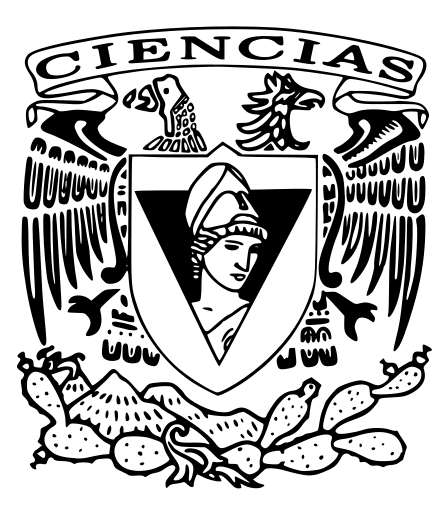
\includegraphics[scale=0.40]{1.png}	
	\end{center}
\newpage
	\begin{center}
		\title {\Huge Problema 1. MCD} 
	\end{center}


Para el máximo común divisor, primero fue necesario definir qué es, y utilizar el algoritmo de Euclides que permite obtener el MCD a partir de ir dividiendo los números entre sí y obtener el residuo, reasignando valores, y repetir. Para ello lo primero que se hizo fue utilizar el comando módulo \% que devuelve el residuo de dos valores y después nadamas se reasignaron valores de nuevo.

\end{document}